%
% The first command in your LaTeX source must be the \documentclass command.
\documentclass[sigconf,authordraft]{acmart}
\usepackage{booktabs}
\usepackage{verbatim}
\usepackage{graphicx}

%
% defining the \BibTeX command - from Oren Patashnik's original BibTeX documentation.
\def\BibTeX{{\rm B\kern-.05em{\sc i\kern-.025em b}\kern-.08emT\kern-.1667em\lower.7ex\hbox{E}\kern-.125emX}}
    
% Rights management information. 
% This information is sent to you when you complete the rights form.
% These commands have SAMPLE values in them; it is your responsibility as an author to replace
% the commands and values with those provided to you when you complete the rights form.
%
% These commands are for a PROCEEDINGS abstract or paper.
\copyrightyear{2018}
\acmYear{2018}
\setcopyright{acmlicensed}
\acmConference[Woodstock '18]{Woodstock '18: ACM Symposium on Neural Gaze Detection}{June 03--05, 2018}{Woodstock, NY}
\acmBooktitle{Woodstock '18: ACM Symposium on Neural Gaze Detection, June 03--05, 2018, Woodstock, NY}
\acmPrice{15.00}
\acmDOI{10.1145/1122445.1122456}
\acmISBN{978-1-4503-9999-9/18/06}

%
% These commands are for a JOURNAL article.
%\setcopyright{acmcopyright}
%\acmJournal{TOG}
%\acmYear{2018}\acmVolume{37}\acmNumber{4}\acmArticle{111}\acmMonth{8}
%\acmDOI{10.1145/1122445.1122456}

%
% Submission ID. 
% Use this when submitting an article to a sponsored event. You'll receive a unique submission ID from the organizers
% of the event, and this ID should be used as the parameter to this command.
%\acmSubmissionID{123-A56-BU3}

%
% The majority of ACM publications use numbered citations and references. If you are preparing content for an event
% sponsored by ACM SIGGRAPH, you must use the "author year" style of citations and references. Uncommenting
% the next command will enable that style.
%\citestyle{acmauthoryear}

%
% end of the preamble, start of the body of the document source.
\begin{document}

%
% The "title" command has an optional parameter, allowing the author to define a "short title" to be used in page headers.
\title[Entity Aspect Linking]{Entity Aspect Linking: Enriching Entity Links with Fine-Grained Knowledge using Entity Salience and Relatedness}

%
% The "author" command and its associated commands are used to define the authors and their affiliations.
% Of note is the shared affiliation of the first two authors, and the "authornote" and "authornotemark" commands
% used to denote shared contribution to the research.
\author{Shubham Chatterjee}
\email{sc1242@cs.unh.edu}
%\orcid{1234-5678-9012}
\affiliation{
 \institution{University of New Hampshire}
  \city{Durham}
 \state{New Hampshire}
}
\author{Jordan Ramsdell}
\email{jsc57@cs.unh.edu}
%\orcid{1234-5678-9012}
\affiliation{
 \institution{University of New Hampshire}
  \city{Durham}
 \state{New Hampshire}
}
\author{Laura Dietz}
\email{dietz@cs.unh.edu}
\affiliation{
 \institution{University of New Hampshire}
  \city{Durham}
 \state{New Hampshire}
}

%
% By default, the full list of authors will be used in the page headers. Often, this list is too long, and will overlap
% other information printed in the page headers. This command allows the author to define a more concise list
% of authors' names for this purpose.
\renewcommand{\shortauthors}{Chatterjee et al.}

%
% The abstract is a short summary of the work to be presented in the article.
\begin{abstract}
Entity linking tools at present provide only coarse-grained information with no knowledge about the different events, topics, roles or in general, aspects of the entity that the mention in the text links to. Entity Aspect Linking is the task of associating an entity link with the correct aspect of the entity mention in the text. Several entity salience and relatedness detectors exist to predict salient entities or relatedness of pairs of entities in text. However, these tools are not trained for a particular task and do not take the queries into account. In this work, we study if and to what extent, such static, off-the-shelf tools can be used in a specific task by utilizing them in the aspect linking task. Our results show that although a static measure of entity salience and relatedness from an off-the-shelf tool works on its own, a supervised combination of these indicators with lexical and semantic features based on the contexts of different sizes around the entity mention provides better results.


%Previous work \cite{nanni2018entity} has shown that a supervised combination of various text and entity features can correctly predict aspects in 70\% of the cases. In this work, we consider the salience of an entity in the aspect (that is, its centrality to the aspect) and its relatedness to other entities and obtain new state-of-the-art results on the task. Moreover, we study the effect of the frequency and relatedness of co-occurring entities with a given entity on the task.
\end{abstract}

% Keywords. The author(s) should pick words that accurately describe the work being
% presented. Separate the keywords with commas.
 %\keywords{entities, entity-aspects, wikification, entity salience, entity relatedness, co-occurring entities}

% This command processes the author and affiliation and title information and builds
% the first part of the formatted document.
\maketitle

\section{Introduction}
\label{sec:Introduction}

%\paragraph{\textbf{Motivation.}} 
%Entity Linking is the task of automatically annotating mentions of entities in text and linking them to their knowledge base entries. Given a sentence such as \textit{Steve Jobs founded the Apple}, entity linking tools first aim to identify the entities in the sentence (such as \textit{Steve Jobs} and \textit{Apple}), and then to disambiguate the entity mentions (does the mention \textit{Apple} refer to the fruit or the company?). Finally, they link the mention to its knowledge base entry. For example, the mention \textit{Apple} would be linked to the knowledge base entry for \textit{Apple\_(Company)} and not \textit{Apple\_(Fruit)}.

Consider a journalist  writing a report on the recent COVID-19 pandemic and who wants to analyse the different angles in which it has been mentioned on social media such as the tweet \textit{Several states are seeing outbreaks of \#COVID19 in meat and poultry processing facilities}. They would not only want to identify and disambiguate the entity \textit{COVID-19}, but also find whether it refers to the \textit{transmission}, \textit{pathology}, or \textit{experimental treatment} of \textit{COVID-19}. Although current entity linking tools \cite{ferragina2010tagme,mendes2011dbpedia,piccinno2014wat} can correctly identify and disambiguate entities, they cannot infer their \textit{aspect} from context. We refer to the different events, roles, and topics which an entity may be related to as an \textit{Entity Aspect}.

%To them, identification and disambiguation of the entity \textit{COVID-19} may not be enough. They would also want to know the different roles the entity plays. For example, does the mention of COVID-19 in the tweet above refer to its \textit{transmission}, \textit{pathology}, or \textit{experimental treatment}? Current entity linking tools \cite{ferragina2010tagme,mendes2011dbpedia,piccinno2014wat} can correctly identify and disambiguate entities in text. However, they cannot infer the correct \textit{aspect} of the entity from the context, such as the aspect of \textit{COVID-19} in the tweet above. %For example, given the sentence, \textit{Boris Johnson is back after recovering from COVID-19}, an entity linking tool can correctly disambiguate and link the mention \textit{Boris Johnson} to its knowledge base entry but cannot infer whether the mention refers to his role as a \textit{Writer at the Daily Telegraph} or as the \textit{Prime Minister of the UK}. In general, an entity mention may be related to several different events, roles, and topics. We refer to each of them as an \textit{Entity Aspect}. 

\textbf{Task.} Given an entity-mention $E_M$ in a specific context $C$ such a tweet, sentence or paragraph, and a set of $N$ predefined aspects $A_{E_M} = \{A_1, A_2, A_3, \cdots, A_N\}$ along with their contents, that capture the addressed topic, link the mention to an aspect $A_i \in A_{E_M}$.

%\paragraph{\textbf{Entity Salience.}} 
Moreover, we would also like to link the entity to the aspect with a content in which the entity is \textit{salient}, that is, \textit{central} to the discussion and not just mentioned on the side. For example, given the sentence \textit{Boris Johnson is back after recovering from COVID-19}, we would not only like to link the entity mention \textit{Boris Johnson} to the aspect \textit{Prime Minister of the UK}, but also to one whose content is a passage like Passage 2 rather than Passage 1 below, because Passage 2 discusses how the entity \textit{Boris Johnson} in his role as the Prime Minister of the UK is affecting the pandemic situation whereas Passage 1 just mentions the entity on the side. We hypothesize that entity salience is a useful indicator of aspects for entities. We use SWAT \cite{swat}  to find the salience of an entity in text. Given some text, SWAT outputs the entities along with their salience scores in the text.
\begin{quote}
\textbf{Passage 1.} The British government came under heightened pressure to disclose details about a secretive scientific advisory group after a report on Friday that a top political aide to Prime Minister Boris Johnson had taken part in the group’s meetings on the coronavirus pandemic. \footnote{https://www.nytimes.com/2020/04/25/world/europe/uk-dominic-cummings-sage-coronavirus.html}\\
\textbf{Passage 2.} British Prime Minister Boris Johnson is resisting growing calls to reopen the UK from its lockdown because he is still so “frightened” from his own near-fatal brush with the bug, according to a report \footnote{https://nypost.com/2020/04/21/boris-johnson-too-frightened-to-ease-uk-coronavirus-lockdown/}.
\end{quote}






%Consider the two passages below from two news articles about the entity \textit{Boris Johnson} which address his role as the \textit{Prime Minister of the UK} and his response to the recent COVID-19 pandemic.
%\begin{quote}
%\textbf{Passage 1.} The British government came under heightened pressure to disclose details about a secretive scientific advisory group after a report on Friday that a top political aide to Prime Minister Boris Johnson had taken part in the group’s meetings on the coronavirus pandemic. \footnote{https://www.nytimes.com/2020/04/25/world/europe/uk-dominic-cummings-sage-coronavirus.html}\\
%\textbf{Passage 2.} British Prime Minister Boris Johnson is resisting growing calls to reopen the UK from its lockdown because he is still so “frightened” from his own near-fatal brush with the bug, according to a report \footnote{https://nypost.com/2020/04/21/boris-johnson-too-frightened-to-ease-uk-coronavirus-lockdown/}.
%\end{quote}
%We notice that Passage 2 discusses how the entity \textit{Boris Johnson} in his role as the Prime Minister of the UK is affecting the pandemic situation, whereas Passage 1 just mentions the entity on the side. The entity is central to the discussion in Passage 2 whereas in Passage 1, it is not. We say that \textit{Boris Johnson} is \textit{salient} in Passage 2. Hence, by \textit{salient}, we mean that the entity is \textit{central} to the text in which it is mentioned. 

%Consider the following sentence from a new article about \textit{Boris Johnson}.

%\begin{quote}
    %\textit{Boris Johnson, perhaps the world's most famous coronavirus patient, was back at work Monday — after spending the worst of Britain's epidemic sidelined, first in self-isolation, then struggling to breathe in the hospital, and later in recovery in the countryside \footnote{https://www.washingtonpost.com/world/europe/boris-johnson-returns-to-work-after-missing-worst-of-coronavirus-epidemic/2020/04/27/95b590ea-8630-11ea-81a3-9690c9881111_story.html}}.
%\end{quote}

%In a sentence such as the one above, we would not only prefer to link the mention \textit{Boris Johnson} to the aspect \textit{Prime Minister of the UK}, but also to one whose content is a passage like Passage 2 and not Passage 1. We hypothesize that entity salience is a useful indicator of aspects for entities. We use SWAT \cite{swat}  to find the salience of an entity in text. Given some text, SWAT outputs the entities along with their salience scores in the text. For example, using the online demo \footnote{https://swat.d4science.org/}, given the two passages above, SWAT correctly predicts \textit{Boris Johnson} as salient in Passage 2 (Score = 0.6), and non-salient in Passage 1 (Score = 0.15). 

%\paragraph{\textbf{Entity Relatedness. }}
\textit{Entity Relatedness} is a measure of how strongly related two entities are. For example, given the entities, \textit{Boris Johnson}, \textit{Theresa May}, and \textit{Donald Trump}, one would say that \textit{Boris Johnson} is more strongly related to \textit{Theresa May} than to \textit{Donald Trump} because both \textit{Boris Johnson} and \textit{Theresa May} are British politicians and had some role in Brexit. We hypothesize that an aspect mentioning many related entities to the target entity (the entity we are trying to aspect link), is a good candidate aspect for the target entity. 
We use the Entity Relatedness system from WAT \cite{piccinno2014wat} to find relatedness between pairs of entities. Given a list of entities, WAT provides the relatedness measure between every pair of entities in the list. 
%For example, given the entity list consisting of \textit{Boris Johnson}, \textit{Theresa May} and \textit{Donald Trump}, WAT predicts the relatedness between every pair of entities as follows:
%\begin{quote}
%    (\text{Boris Johnson}, \text{Donald Trump}) = 0.37, \\
%    (\text{Theresa May},\text{Donald Trump})    = 0.38, \\
%    (\text{Boris Johnson}, \text{Theresa May})  = 0.67
%\end{quote}

%\paragraph{\textbf{Co-occurring Entities.}}
\textit{Co-occurring entities} are entities which co-occur with a given entity in a particular context such as a sentence, passage or article. For example, entities which might co-occur with \textit{Boris Johnson} in a passage may be \textit{Theresa May}, \textit{United Kingdom} and \textit{Brexit}. We study the role of such co-occurring entities on the aspect linking task by comparing whether the frequency or relatedness of these co-occurring entities to a given entity is a better indicator of aspects and under what conditions they work. 

%Nanni et al. \cite{nanni2018entity} have shown that a supervised combination of various text and entity features based on embeddings of the words and entities from various sources (context of mention, content of Wikipedia page of the mention, etc) is able to correctly predict aspects in 70\% of the cases. In this work, we build on their work and use entity salience and relatedness based features in supervised setting with some lexical and semantic features used in \cite{nanni2018entity} and show that this leads to significant improvements in results on the task.

\textbf{Contributions.} In this paper, we study whether we can utilize an off-the-shelf, static (not trained for the task) entity salience and relatedness detector in our work and show that a supervised combination of these indicators along with some lexical and semantic features derived from contexts of varying sizes can outperform several baselines. 

%and analysis of the conditions under which these entity salience and relatedness work versus do not work. we show that although entity salience and entity relatedness can work on their own, a supervised combination of these indicators along with some lexical and semantic features derived from contexts of all sizes can outperform several baselines and the current state-of-the-art on the task for contexts larger than a sentence.
%Nanni et al. \cite{nanni2018entity} have shown that a supervised combination of various text and entity features derived from contexts of different lengths such as the sentence, paragraph or section surrounding the entity mention, is useful in the task. 
%Nanni et al. \cite{nanni2018entity} have presented results on the task using contexts of different sizes (such as the sentence, paragraph or section surrounding the entity mention) separately. In particular, they show that considering the sentence as the context around the entity mention can help predict aspects in 70\% of the cases. However, considering a context size larger than a sentence (such as a paragraph or a section) can degrade performance. Their work is a study on using these contexts of different sizes separately, that is, they do not consider sentence or paragraphs, when they consider the section.

%The work by Nanni et al. \cite{nanni2018entity} is well suited for aspect linking entity mentions in short texts such as tweets. However, it is not particularly suitable when larger text such as a newspaper article is considered. In this work, we study how to use a context size larger than a sentence for aspect linking. In this regard, we study the role of entity salience, entity relatedness and co-occurring entities on the task.

%in many cases, more data is available than just the sentence mentioning the entity. For example, in a newspaper article, Nanni et al.\cite{nanni2018entity} show that using this entire article as the context of the entity does not perform as well as using just the sentence mentioning the entity. However, ignoring this article would mean that we disregard useful information from the other entities in the article. In this work, we study how to use a context size larger than a sentence for aspect linking. In this regard, we study the role of entity salience, entity relatedness and co-occurring entities on the task.

%This paper studies the role of entity salience and relatedness on the aspect linking task. We study how these indicators can help and under what conditions they work. We show that using these indicators alone may not be useful but a supervised combination of salience and relatedness based features along with some lexical and semantic features outperforms the current state-of-the-art on the task. We also study the effect of using the frequency and relatedness of contextual entities on the task.

%Our contributions are as follows.
%\begin{enumerate}
%    \item We show that although entity salience and entity relatedness can work on their own, a supervised combination of these indicators along with some lexical and semantic features derived from contexts of all sizes can outperform several baselines and the current state-of-the-art on the task for contexts larger than a sentence to achieve better results.
%    \item We present a detailed study and analysis of the conditions under which these entity salience and relatedness work versus do not work. 
%\end{enumerate}

%\paragraph{\textbf{Outline.}} The remainder of this paper is organized as follows. Section \ref{sec:Related Work} discusses some related work on the topic. Section \ref{sec:Approach} presents our proposed method in detail. Section \ref{sec:Evaluation} presents a quantitative evaluation of our work. Finally, we conclude the paper with Section \ref{sec:Conclusion}.

\section{Related Work}
\label{sec:Related Work}
%\paragraph{\textbf{Entity Linking.}}
The task of Entity Linking is to link the mention of an entity in text to a knowledge base entry. Current entity linking systems such as TagMe \cite{ferragina2010tagme}, DBPedia Spotlight \cite{mendes2011dbpedia}, %Babelfy \cite{babelfy} 
and WAT \cite{piccinno2014wat} examine the context around the entity to disambiguate the entity mention. 
%For example, in the sentence \textit{Steve Jobs founded Apple}, the system would predict from the context that the mention \textit{Apple} refers to the company but in the sentence \textit{The apple fell on Newton's head}, the mention \textit{apple} refers to the fruit. 
More recently, systems have been developed to produce embeddings of entities from text and knowledge graphs \cite{ristoski2016rdf2vec,yamada2016joint} and for entity disambiguation and linking \cite{yamada2017learning}. 

%In this work, we aim to further enrich an entity link with the correct aspect of the entity mention in the text. We treat the sections from the Wikipedia page of the entity mention as different aspects of the entity and given an entity mention along with the sentence, paragraph and section context, try to link it to the correct section (that is, aspect).

%\paragraph{\textbf{Entity Aspect Linking using Sections.}} 
%The following works try to map entities or passages to Wikipedia sections, similar to how we want to map an entity to a Wikipedia section.

Fetahu et al. \cite{fetahu2015automated} enrich Wikipedia sections with news-article references in two steps: article-entity placement and article-section placement.
%First, they suggest news articles to Wikipedia entities (article-entity placement step) and Second, they find the exact section in the entity page where the article must be placed (article-section placement step).
Banerjee et al. \cite{banerjee2015wikikreator} seek to improve Wikipedia stubs by generating content for each section automatically using a text classifier which uses topic distribution vectors, followed by by an abstractive summarization step to generate section-specific summaries for Wikipedia stubs.
%Their system is based on a text classifier which uses topic distribution vectors to assign content from the web to various sections on a Wikipedia article. This is followed by an abstractive summarization step where section-specific summaries for Wikipedia stubs are generated.
%Reinanda et al. \cite{reinanda2016document} present a method for document filtering for long-tail entities, which is based on using aspect-features to identify relevant documents. 
Nanni et al. \cite{nanni2018entity} define each section of the Wikipedia page of the entity as an aspect following \cite{fetahu2015automated,banerjee2015wikikreator} and present a learning-to-rank based method which uses both lexical and semantic features derived from various contexts such as the sentence, paragraph and section where the entity is mentioned in text. 

%In their work, they present a learning-to-rank based method which uses both lexical and semantic features derived from various contexts such as the sentence, paragraph and section where the entity is mentioned in text. They use two types of feature-vectors: (a) Word Vector Models, which consider the symbolic representation of each word as a token using TF-IDF and BM25, and rank aspects using the header, content and entity representations and, (b) Distributional Semantic Models, where each word/entity is represented by its embedding for ranking aspects with header and content representations. They show that using lexical and semantic features with different context sizes improves performance over several established baselines. They also showed the usefulness of their method on three downstream applications.  


%They present a learning-to-rank based method which uses both lexical and semantic features derived from various contexts such as the sentence, paragraph and section where the entity is mentioned in text and show that this improves performance over several established baselines. 

%In this work, we adopt the same definition of aspects as Nanni  et al. \cite{nanni2018entity} and use their dataset. However, as stated in Section \ref{sec:Introduction}, our work is different in that we consider the role of entity salience, entity relatedness and co-occurring entities for improving performance when more data (for example, in the form of a newspaper article), is available. We show that ignoring the sentence and paragraph level information in an article is detrimental to aspect linking an entity mention in the article, and that a supervised combination of lexical and semantic features from contexts of various sizes, along with salience and relatedness features, achieves state-of-the-art results.



In our work, we adopt the same definition of aspects as Nanni  et al. \cite{nanni2018entity} and use their dataset. However, we consider the role of entity salience and relatedness and show that a supervised combination of lexical and semantic features from different contexts, with salience and relatedness features can improve upon several established baselines.

%\paragraph{\textbf{Using Co-occurring Entities}}
%The following works use entities which co-occur with a given entity in two different tasks and show their effectiveness on the task. Dalton et al. \cite{dalton2014entity} present the Entity Context Model (ECM) in their work on Entity Query Feature Expansion. They use the ECM to derive a distribution over words in the context of an entity and co-occurring entities with the entity.Chatterjee et al. \cite{chatterjee2019why} present the Entity Context Document (ECD) in their work in Entity Support Passage Retrieval.For a given query and entity, they try to find a passage which explains to the user, the relationship between the query and the entity. They show that using frequently co-occurring entities with the target entity (the entity about which the support passage needs to be found) is useful in the task.Following the idea about using co-occurring entities in \cite{dalton2014entity, chatterjee2019why}, we study the effect of using the frequency and relatedness of co-occurring entities on the entity aspect linking task. In particular, we study whether using the frequency of co-occurrence or the relatedness of the co-occurring entities to a given entity is a better indicator of aspects.

\section{Approach}
\label{sec:Approach}
Our goal is to enrich entity links with fine-grained aspects of the entities. In this work, we consider whether a static measure of entity salience and relatedness which has not been trained for this task can help. We refer to the entity that we are trying to aspect link as the target entity.

%To study the role of entity salience, entity relatedness and co-occurring entities, we describe below several ranking strategies based on these and later combine them in a learning-to-rank system. In all our discussions, we refer to the entity that we are trying to aspect link as the target entity.

\subsection{Features}
\label{subsec:Features}

\subsubsection{Entity salience based features}
\label{subsubsec:Entity salience based features}
We use SWAT \cite{swat} to find salience of entities in text. Given a text, SWAT returns the entities in the text along with their salience scores.
\begin{enumerate}
    \item \textbf{Salience of Entity Mention in aspect (Sal-EM).} Score of the aspect is equal to the salience score of the entity mention in the aspect if the entity is salient, and zero otherwise.
    
    \item \textbf{Salient Entities in Context (SEC).} Score an aspect by summing over the salience score of entities $e \in E$, where $E = E_A \cap E_C$, $E_A =$ aspect entities, and $E_C =$ salient entities in sentence, paragraph and section context.
    
    %We use the sentence, paragraph and section context around the entity mention to get the set of salient entities $E_C$ in the context using SWAT. We then find the set of entities $E_A$ in the aspect using WAT\cite{piccinno2014wat}. We then find how many entities in the aspect overlap with the salient entities in the context, $E = E_A \cap E_C$. We then score an aspect by summing over the salience score of common entities in $E$. If no overlap is found, the aspect score is zero.
    
    %\item \textbf{Salient entities in context.} We use the sentence, paragraph and section context around the entity mention to get the set of salient entities $E_C$ in the context using SWAT. We then find the set of entities $E_A$ in the aspect in two ways: (a) Salient entities using SWAT \cite{swat} \textbf{(SEC-swat)} and (b) All entities using WAT \textbf{(SEC-wat)} \cite{piccinno2014wat}. We then find how many entities in the aspect overlap with the salient entities in the context, $E = E_A \cap E_C$. We then score an aspect by summing over the salience score of common entities in $E$. If no overlap is found, the aspect score is zero. Note, that the context referred to here is the local context of the target entity such as the sentence or paragraph in which the target entity occurs. Later, in Section \ref{subsubsec:Features based on contextual entities}, we use the term contextual entities to refer to other entities which co-occur with the target entity in the entire document collection. The use of the term \textit{contextual} in Section \ref{subsubsec:Features based on contextual entities} should not be confused with the use of the term \textit{context} here.
    
    \item \textbf{All Entities in Context (AEC).} Same as \ref{subsubsec:Entity salience based features}(2) above, but use both salient and non-salient entities from SWAT for $E_C$.
    
    %To investigate the extent to which salient entities can affect the performance, we also experiment with using both salient and non-salient entities from SWAT for $E_C$ in \ref{subsubsec:Entity salience based features}(2) above. 
\end{enumerate}


\subsubsection{Entity relatedness based features.} 
\label{subsubsec:Entity relatedness based features}
We use WAT \cite{piccinno2014wat} to find relatedness of two entities. Given a list of entities, WAT returns the relatedness between every pair in the list.


\textbf{Co-occurring entities with an entity from context.}
For every entity $e$ in the sentence, paragraph and section context around the target entity $e_T$, we derive a distribution over co-occurring entities with $e$ using the frequency of co-occurrence and the relatedness of co-occurring entities to $e$. We may treat this distribution as the the conditional probability distribution $P(e' \vert e)$. To find the co-occurring entities, we use the Entity Context Document (ECD) \cite{chatterjee2019why} for $e$. The ECD is created by first retrieving a candidate set of passages using $e$ as the query and then concatenating all passages which mention $e$.
%We find the set of all entities $E$ in the sentence, paragraph and section context around the target entity. For every entity $e \in E$, we derive a distribution over the co-occurring entities $e'$ with $e$. This is done using an initial candidate set of passages retrieved using the entity $e$ as the query (using Lucene defualt BM25) from an index of passages from the TREC Complex Answer Retrieval \cite{dietz2018trec} track dataset. Then we concatenate all passages in the candidate set which mention the entity $e$ as in \cite{dalton2014entity,chatterjee2019why}, to get a composite document of all passages mentioning $e$. We call this composite document as an Entity Context Document (ECD) following Chatterjee et al. \cite{chatterjee2019why}. All entities in this ECD are the co-occurring entities with $e$. We then derive a distribution over co-occurring entities with $e$ in two ways: (a) frequency of co-occurrence, and (b) relatedness of each co-occurring entity $e'$ to the entity $e \in E$. We may treat this distribution as the the conditional probability distribution $P(e' \vert e)$, the conditional probability of seeing the co-occurring entity $e'$ provided that we have already seen the target entity $e$. 
We score an aspect $A$ in following ways.

\begin{enumerate}
    \item \textbf{Simple Frequency Distribution (SF-Dist).} 
    Score an aspect using
    \begin{equation}
    \label{eq:score-aspect-using-simple-freq-dist}
        \text{Score(A)} = \sum_{e' \in A}P(e' \vert e)
    \end{equation}
    where $e'$ is an entity in the aspect $A$ which also frequently co-occurs with $e$, $e$ is an entity from the context around the target entity $e_T$, and $P( e' \vert e)$ is the frequency distribution over co-occurring entities.
    
    %We score aspects using frequently co-occurring entities with an entity $e$ from the sentence, paragraph and section context around the target entity, which also occur in the aspect content. Formally,:
    %\begin{equation}
    %\label{eq:score-aspect-using-simple-freq-dist}
    %    \text{Score(A)} = \sum_{e' \in A}P(e' \vert e)
    %\end{equation}
    %where $e'$ is an entity in the aspect $A$ which also frequently co-occurs with $e$, $e$ is an entity from the context around the target entity, and $P( e' \vert e)$ is the frequency distribution over co-occurring entities.
    
    \item \textbf{Weighted Frequency Distribution (WF-Dist).} 
    Same as \ref{subsubsec:Entity relatedness based features}(1) above, but weigh each probability by the relatedness of $e'$ to the target entity $e_T$.
    
    %Our intuition is that co-occurring entities which are more related to the target entity should contribute more to the final aspect scores. To investigate how relatedness of co-occurring entities affects the aspect scores, we experiment with scoring an aspect $A$ using a weighted sum of frequencies of entities $e'$ in the aspect, weighted by the relatedness of $e'$ to the target entity $e_T$. Formally,
%\begin{equation}
%\label{eq:score-aspect-using-weighted-freq-dist}
%    \text{Score(A)} = \sum_{e' \in A} \text{Relatedness}(e', e_T) \times P(e' \vert e)
%\end{equation}
%where $e'$ is an entity in the aspect $A$ which also frequently co-occurs with $e$, $e_T$ is the target entity, $e$ is an entity from the context around the target entity $e_T$, and $\text{Relatedness}(e', e_T)$ is found using WAT \cite{piccinno2014wat}.

\item \textbf{Relatedness Distribution (Rel-Dist).} 
Same as \ref{subsubsec:Entity relatedness based features}(1), but use relatedness of $e'$ to $e$ to find $P( e' \vert e)$.

%Same as \ref{subsubsec:Co-occurring entities based features}(1), but we use the relatedness measure between a co-occurring entity $e'$ and an entity $e$ from the context around the target entity to derive the distribution $P( e' \vert e)$.
\end{enumerate}

\textbf{Co-occurring entities with the target entity.} 
We use two sources of co-occurring entities with the target entity $e_T$: Entity Context Document (\textbf{ECD}) for $e_T$ and the Wikipedia page (\textbf{Wiki}) of $e_T$. We then score an aspect using the co-occurring entities with $e_T$ in two ways.

    
\begin{enumerate}
    \item Use Equation \ref{eq:score-aspect-using-simple-freq-dist} with either frequency distribution \textbf{(SF-Dist-ECD)} or relatedness distribution \textbf{(Rel-Dist-ECD/Rel-Dist-Wiki)} over co-occurring entities to score an aspect.
        
    \item Retrieval Score of Aspect (\textbf{RS-Asp}). We treat the target entity $e_T$ as the query and expand the query using top-20 (according to frequency (\textbf{Freq}) and relatedness (\textbf{Rel})) entities from the ECD/Wikipedia page for $e_T$. We then retrieve aspects from an aspect index for $e_T$ (\textbf{RS-Asp-Freq-ECD/RS-Asp-Rel-ECD/RS-Asp-Rel-Wiki}). We experiment with the combinations of the following retrieval models: BM25 (default Lucene), Language Models with Jelinek-Mercer (LMJM) smoothing $(\lambda = 0.4)$, and Language Models with Dirichlet (LMDS) smoothing, and the following expansion models: RM1 and RM3.
\end{enumerate}
    



%We derive a distribution over co-occurring entities $e'$ with the target entity $e_$ in two ways: (a) Frequency distribution and (b) Relatedness distribution. We then score the aspects in two ways: 
%\begin{enumerate}
%    \item \textbf{Entities in aspect.} Score an aspect with Equation \ref{eq:score-aspect-using-simple-freq-dist} using either the frequency distribution \textbf{(Asp-Ent-Freq-Dist)} or relatedness distribution \textbf{(Asp-Ent-Rel-Dist)}
    
%     \item \textbf{Retrieval score of an aspect (RS-Asp).} For a given target entity, we treat the target entity as a query and expand the query using the top-20 entities from the distribution obtained above. We then score candidate aspects for the target entity by retrieving aspects from an in-memory aspect-index for the target entity. We experiment with the combinations of the following retrieval models: BM25 (default Lucene), Language Models with Jelinek-Mercer (LMJM) smoothing $(\lambda = 0.4)$, and Language Models with Dirichlet (LMDS) smoothing, and the following expansion models: RM1 and RM3.
%\end{enumerate}


%\subsubsection{Wikipedia page entity based features}
%\label{subsubsec:Wikipedia page entity based features}
%We derive a distribution over all entities on the Wikipedia page of the target entity using the relatedness of the entities to the target entity. We score an aspect using this distribution in two ways:
%\begin{enumerate}
%    \item \textbf{Entities in aspect (Asp-Ent-Wiki).} Score an aspect using this distribution using Equation \ref{eq:score-aspect-using-simple-freq-dist}.
    
%    \item \textbf{Retrieval score of an aspect (RS-Asp-Wiki).} For a given target entity, we treat the target entity as a query and expand the query using the top-20 related entities from the Wikipedia page of the target entity. We then score candidate aspects for the target entity by retrieving aspects from an in-memory aspect-index for the target entity. We experiment with the combinations of the same retrieval and expansion models as when retrieving aspects using co-occurring entities with a target entity above.
%\end{enumerate}


\subsubsection{Lexical and Semantic features}
\label{subsubsec:Lexical and Semantic features} 
We re-implemented the lexical and semantic features from Nanni et al.\cite{nanni2018entity}. To give a brief recap, Nanni et al.\cite{nanni2018entity} consider three types of aspect representations and rank aspects based on similarity of mention in context to:(1) Header, (2) Content and, (3) Entity overlap with each section on the Wikipedia page of the entity. They use four methods to derive features from the aspect representations above: (1) TF-IDF, (2) BM25, (3) Word Embeddings and, (4) Entity Embeddings.

\begin{comment}
We give a brief overview of the same again for reference. 

Nanni et al.\cite{nanni2018entity} consider three types of aspect representations for finding its similarity to the entity mention in context. 

\textbf{Header.} Rank aspects based on similarity of the mention in context to the header of each section in the Wikipedia page.

\textbf{Content.} Rank aspects based on the similarity between the mention in context and the content of each section of the Wikipedia page of the entity.

\textbf{Entity.} Overlap of entities mentioned in the context of the entity mention and the content of a section on the Wikipedia page of the entity.

They use the following features to rank aspects using the representations above.

\textbf{TF-IDF.} Cosine similarity between the TF-IDF (logarithmic, L2-normalized) vector of contextual mention and aspect.

\textbf{BM25.} Rank aspect representations using the contextual mention as a query using BM25 ($k_1=2, b=0.75)$.

\textbf{Word Embeddings.} Cosine similarity between the mention in context and the aspect using pre-trained GloVe \cite{pennington2014glove} embeddings of dimension 300. 

\textbf{Entity Embeddings.} Use 500 dimensional RDF2Vec \cite{ristoski2016rdf2vec} embeddings to embed entities in the context of the entity mention and a section from the Wikipedia page of the entity, then compute
the document vector using the TF-IDF of an an entity in context of the entity mention and its embedding.
\end{comment}
 


\section{Evaluation}
\label{sec:Evaluation}
%In this section, a quantitative evaluation of our system is presented on the entity-aspect dataset from Nanni et al.\cite{nanni2018entity}. We begin by presenting some research questions pertaining to three broad components of our system: Entity Salience, Entity Relatedness and Co-occurring entities, which our experiments aim to address(Section \ref{subsec:Research Questions}). We then describe our experimental settings (Section \ref{subsec:Evaluation Paradigm}), followed by the baselines (Section \ref{subsec:Baselines}). We end this section with a discussion of our experiments and results (Section \ref{subsec:Results}).

\subsection{Research Questions}
\label{subsec:Research Questions}

\begin{itemize}
\item[\textbf{RQ1}] Does entity salience affect the task? If yes, then to what extent?
%\item[\textbf{RQ3}] What is the effect of using salient entities versus all (salient + non-salient) entities? 
\item[\textbf{RQ2}] Does entity relatedness affect the task? If yes, then to what extent? 
%\item[\textbf{RQ5}] When using co-occurring entities, is a global context around the entity mention (obtained from all passages mentioning the entity) better than using a local context (such as a sentence, paragraph, section or Wikipedia article)? In each case, is frequency or relatedness of co-occurring entities a better indicator of a good aspect?
\item[\textbf{RQ3}] Is the frequency or relatedness of co-occurring entities a better indicator of a good aspect?
\end{itemize}

\subsection{Evaluation Paradigm}
\label{subsec:Evaluation Paradigm}

%\paragraph{\textbf{Datasets.}}
We use the Entity Aspect Linking dataset from Nanni et al.\cite{nanni2018entity} to evaluate our methods. It consists of 201 entity mentions from Wikipedia along with their sentence, paragraph and section context and a list of candidate aspects for the mention, along with a ground truth file which maps a mention to the correct aspect.  We use the TREC Complex Answer Retrieval track \cite{dietz2018trec}\footnote{\url{http://trec-car.cs.unh.edu}} dataset as a source of passages when building the Entity Context Document in Section \ref{subsubsec:Co-occurring entities based features}. It consists of an entity linked corpus consisting of paragraphs from the entire English Wikipedia. We use Precision at 1 (P@1) and Mean Reciprocal Rank (MRR) as our evaluation metrics. We apply our methods to produce an aspect ranking for every entity mention. We then treat each ranking as a feature and perform 5-fold cross validation using learning-to-rank (L2R) with Coordinate Ascent optimized for Precision at 1 (P@1). We use RankLib\footnote{Dang, V. "The Lemur Project-Wiki-RankLib." Lemur Project,[Online]. Available: \url{http://sourceforge. net/p/lemur/wiki/RankLib}.} for this purpose. 

%\paragraph{\textbf{Ground Truth.}} 
%The dataset from Nanni et al. \cite{nanni2018entity} contains a ground truth file which maps a mention to the correct aspect. The TREC Complex Answer Retrieval track \cite{dietz2018trec} dataset contains both passage and entity ground truth data, however in our work, we do not need to use them. 

%\paragraph{\textbf{Evaluation Metrics.}} 
%We use Precision at 1 (P@1) and Mean Reciprocal Rank (MRR) as our evaluation metrics. %---omitted results will be made available in our online appendix upon acceptance.   

%\paragraph{\textbf{Machine Learning.}}
%We apply our methods to produce an aspect ranking for every entity mention. We then treat each ranking as a feature and perform 5-fold cross validation with a listwise learning-to-rank (L2R) method (Coordinate Ascent) optimized for Precision at 1 (P@1). We use RankLib\footnote{Dang, V. "The Lemur Project-Wiki-RankLib." Lemur Project,[Online]. Available: \url{http://sourceforge. net/p/lemur/wiki/RankLib}.} for this purpose. 

\subsection{Baselines}
\label{subsec:Baselines}

\textbf{Baseline 1: Nanni et al.} We re-implement all features from Nanni et al. \cite{nanni2018entity} and use a supervised combination of sentence, paragraph and section context features as our baselines. \\
\textbf{Baseline 2: Size.} We consider the length of each section (in number of tokens) and link the entity-mention to the longest. \\
%\textbf{Baseline 3: Content Overlap.} Overlap between the tokens in the sentence, paragraph and section context of the mention. \\
%\textbf{Baseline 4: Entity Overlap.} Overlap between the entities in the sentence, paragraph and section context of the mention. \\

\subsection{Results}
\label{subsec:Results}
The most interesting results are presented in Table \ref{tab:Results}. Due to space constraints other results were moved to the online appendix for this paper. Below, we discuss each of the research questions presented in Section \ref{subsec:Research Questions}.
%Below, we discuss results from our experiments with respect to the three broad components of our system: entity salience, entity relatedness and co-occurring entities, and answer the research questions presented in Section \ref{subsec:Research Questions}.


\begin{figure}
    \centering
    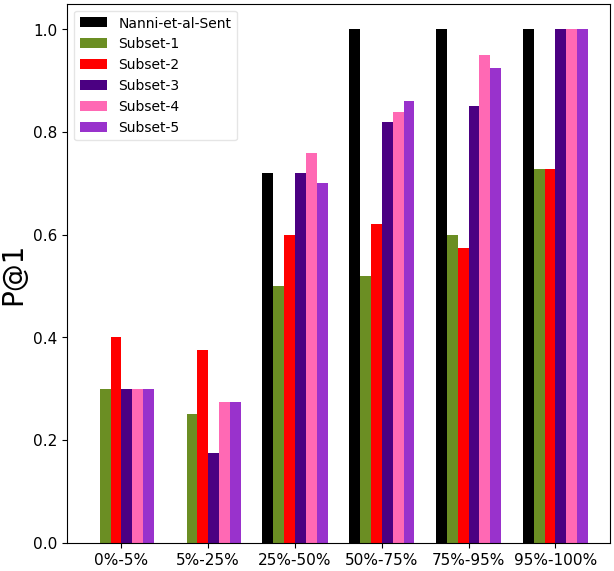
\includegraphics [scale=0.5]{plot-cropped.png}
    \caption{Difficulty-test for P@1, comparing Nanni et al.(Sentence) to various L2R systems.}
    \label{fig:difficulty-plot}
\end{figure}


\begin{table}[t]
    \caption{Performance with standard error of individual features and combined with L2R, including subsets/ablations.}
    \label{tab:Results}
    \scalebox{0.9}{
    \begin{tabular}{@{}lllll@{}}
        \toprule
        Method & 
        P@1 &
        MRR \\ 
        
        \midrule
        
     
      
     
      Nanni et al. (Sentence)&  
      0.67$\pm$0.03&
      0.79$\pm$0.02
      \\
      
      
    
      Nanni et al. (Paragraph)&  
      0.64$\pm$0.03&
      0.78$\pm$0.03
      \\
      
      Nanni et al. (Section)&  
      0.53$\pm$0.03&
      0.71$\pm$0.03
      \\
      
     
      Size &
      0.39$\pm$0.03&
      0.60$\pm$0.03
      \\
      
      \midrule
      
     
      Sal-EM   &   
      0.19$\pm$0.03 &
      0.46$\pm$0.03
      \\
      
      
      
      SEC (Sentence)  &    
      0.23$\pm$0.03 &
      0.53$\pm$0.03
      \\
      
      
      AEC (Sentence)   &    
      0.51$\pm$0.03 &
      0.70$\pm$0.03
      \\
       \midrule
      
     
      SF-Dist (Sentence)   &    
      0.54$\pm$0.03 &
      0.72$\pm$0.03
      \\
      
     
      WF-Dist (Sentence)  &    
      0.49$\pm$0.03 &
      0.67$\pm$0.03
      \\
      
      
      Rel-Dist (Sentence)  &    
      0.43$\pm$0.03 &
      0.62$\pm$0.03
      \\
       \midrule
      
    
      SF-Dist-ECD   &    
      0.35$\pm$0.03 &
      0.59$\pm$0.03
      \\
      
      
      Rel-Dist-ECD  &    
      0.36$\pm$0.03 &
      0.60$\pm$0.03
      \\
      
     
      RS-Asp-Freq-ECD (LMJM + RM1)  &     
      0.35$\pm$0.03 &
      0.59$\pm$0.03
      \\
      
       
      RS-Asp-Rel-ECD (LMJM + RM1) &     
      0.40$\pm$0.03 &
      0.60$\pm$0.03
      \\
       \midrule
      
      
      Rel-Dist-Wiki  &    
      0.37$\pm$0.03 &
      0.60$\pm$0.03
      \\
      
      
       
      RS-Asp-Rel-Wiki (BM25 + RM3)  &     
      0.39$\pm$0.03 &
      0.61$\pm$0.03
      \\
      \midrule
      
       Subset-1 (Only Relatedness) &
      0.48$\pm$0.03 &
      0.68$\pm$0.03
      \\
      
      
      Subset-2 (Only Salience) &
      0.59$\pm$0.03 &
      0.72$\pm$0.03
      \\
      
       Subset-3 (Rel. + Lex. + Sem.) &
      0.66$\pm$0.03 &
      0.78$\pm$0.03
      \\
      
       Subset-4 (Sal + Lex. + Sem.) &
      
      0.72$\pm$0.03 &
      0.82$\pm$0.03
      \\
      
      
      Subset-5 (Sal. + Rel. + Lex. + Sem.) &
      0.70$\pm$0.03 &
      0.81$\pm$0.03
      \\
     
      
      

     
      
       \bottomrule
    \end{tabular}
    }
\end{table}


%\subsubsection{Entity Salience}
%\label{subsubsec:Entity Salience}
\textbf{RQ1: Entity Salience.}
%\paragraph{\textbf{Observations.}}
We observe from Table \ref{tab:Results} that a supervised combination of all salience features (Subset-2) outperforms 2 of the 3 baselines, whereas a combination of all salience features with the lexical and semantic features (Subset-4) outperforms all baselines. However, considering all entities (salient and non-salient) in the context (AEC Sentence) performs better than considering only the salient entities (SEC Sentence). We also find that in Subset-2, learning-to-rank always places maximum weight on the AEC methods.
%\paragraph{\textbf{Discussions.}}
These observations show the effectiveness of using salience. However, they also indicate that considering non-salient entities together with the salient ones help improve performance. We manually confirmed that SWAT correctly identifies salient entities in text. However, SWAT returns more empty results when asking for only salient entities than when asking for all (salient or otherwise) entities. For example, using the sentence context of an entity mention, it returns an empty result for 100 of the 201 entity mentions when asked for only the salient entities and 13 of 201 entity mentions when asked for all  entities. This shows the limitations in SWAT and why the results obtained using \textit{SEC (Sentence)} is lower than \textit{AEC (Sentence)}.  Our intuition is that the other entities, although non-salient, have some inherent semantic meaning and hence considering them together with the salient entities helps the task. %This is the case for the paragraph and section contexts too but we do not show the results here due to space constraints. 

To investigate the extent to which salience helps, we divide the entity mentions  into different levels of difficulty according to the performance (P@1) of the \textit{Nanni et al. (Sentence)} method, with the 5\% most difficult queries for this method to the left and the 5\% easiest ones to the right, and compare the performance with the \textit{Subset-4}. The results are shown in Figure \ref{fig:difficulty-plot}. We observe that whenever it is difficult to perform the task using \textit{Nanni et al. (Sentence)}, entity salience supports our L2R system (Subset-2 and Subset-4).

\textbf{Conclusions.}
Entity salience does indeed affect the task positively by learning information which is complimentary to the lexical and semantic features. However, the limitations of SWAT hinder the performance of a system using it.

%We are able to outperform all the baselines with the help of salience and we see that salience helps to boost performance when the queries get difficult. However, SWAT is still limited in its salience detection and this hinders the performance of a system using it. 

\textbf{RQ2: Entity Relatedness.}
%\subsubsection{Entity Relatedness}
%\label{subsubsec:Entity Relatedness}
%\paragraph{\textbf{Observations.}}
We observe from Table \ref{tab:Results} that a supervised combination of all relatedness features (Subset-1) does not perform very well on its own, doing better than only one baseline (Size). However, a combination of relatedness features with the lexical and semantic features (Subset-3) does significantly better than 3 of the 4 baselines. Moreover, a combination of salience and relatedness features with the lexical and semantic features outperforms all baselines. 
%\paragraph{\textbf{Discussions.}}
These observations indicate that entity relatedness does indeed affect the task positively. However, salience is more informative than relatedness as is evident from the superior performance of Subset-2 over Subset-1 and Subset-4 over Subset-3. On further investigation, we found that WAT finds many false positives and false negatives. For example, given the entity list consisting of  \textit{World War I}, \textit{Vietnam War} and \textit{France}, it predicts that \textit{World War I} is related to \textit{Vietnam War} (false positive) but  unrelated to \textit{France} (false negative). This is because WAT does not take the query or the context of the entity into account but makes predictions based on certain graph-based features such as number of inlinks and outlinks to and from a particular entity node in a knowledge graph. Moreover, from the difficulty plot in Figure \ref{fig:difficulty-plot}, we observe that whenever it is difficult to perform the task using \textit{Nanni et al. (Sentence)}, entity relatedness supports our L2R system (Subset-3 and Subset-5).


\textbf{Conclusions.}
Although relatedness of entities by itself may not perform very well, a supervised combination with lexical and semantic features improves performance over several baselines. However, the limitations of WAT hinder the performance of a system using it.

%considering relatedness features in combination with some lexical and semantic features can help the task. However, WAT is limited in its entity relatedness system where it finds many false positives and false negatives.

\textbf{RQ3: Frequency vs Relatedness.}
%\subsubsection{Co-occurring Entities}
%\label{Co-occurring Entities}
From Table \ref{tab:Results}, we observe that ranking aspects using \textit{SF-Dist (Sentence)} outperforms \textit{WF-Dist (Sentence)}, which in turn outperforms \textit{Rel-Dist (Sentence)}). Moreover, \textit{RS-Asp-Freq-ECD} outperforms \textit{RS-Asp-Rel-ECD}. We also find that when L2R is trained on all relatedness features (Subset-1), it places more weight on the features using frequency distribution those using relatedness. These observations indicate that using the frequency of co-occurring entities is more informative than the relatedness. To investigate this further, we evaluate the quality of the intermediate entity rankings produced by using the frequency and relatedness of entities in Sections \ref{subsubsec:Entity relatedness based features}(1) and \ref{subsubsec:Entity relatedness based features}(3) by defining all entities in an aspect as relevant for the aspect. We find that the entity rankings obtained using frequency distribution are indeed better (in terms of Mean Average Precision (MAP)) than those obtained using relatedness. For example, entity ranking obtained using section context and frequency distribution has $\text{MAP}=0.13$ whereas that obtained using relatedness has $\text{MAP}=0.04$. 

\textbf{Conclusions.} Using frequency of co-occurring entities is better than using relatedness because most frequently co-occurring entities are also related but most related entities do not frequently co-occur.

\section{Conclusion}
\label{sec:Conclusion}
This work addresses the task of entity aspect linking and studies the effectiveness of using entity salience and relatedness on the task using two off-the-shelf tools not trained for this task. We show that although these tools have some inherent defects, a supervised combination of salience and relatedness features with lexical and semantic features can outperform several established baselines. In particular, we show that such a supervised combination learns complimentary information which aids the performance of the supervised system. Moreover, we find that using the frequency of co-occurring entities is better than using their relatedness since frequently co-occurring entities are mostly related, but related entities might not co-occur frequently. 

\bibliographystyle{ACM-Reference-Format}
\bibliography{references}
\end{document}

